\documentclass[../manuscript.tex]{subfiles}

\section{Материалы и методы}

\subsection{Вероятностная модель числа прочтений}
При работе с данными секвенирования часто возникает задача оценить матожидание числа прочтений по заданному участку генома. В случае DNA-seq, эта величина описывается простой вероятностной моделью

\begin{figure}[H]
	\centering
	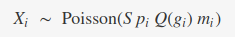
\includegraphics{images/poisson_sequencing_model.png}
	\caption{Вероятностая модель числа прочтений $X_i$ в сегменте $i$ в DNA-seq. $S$ — \textit{scale factor}, $p_i$ — число копий сегмента, $Q(g_i)$ — влияние \textit{GC-состав}, $m_i$ — \textit{bin mappability}}
\end{figure} 

Ниже приведены определения этих факторов:

\begin{definition}[\textit{Scale factor}]
	Число ридов, которые фрагмент ДНК порождает при секвенировании. Эта величина зависит как от \textbf{сложности библиотеки} (матожидание числа различных молекул, которые могут получиться в ходе ПЦР), так и от \textbf{глубины секвенирования} (точное значение зависит от технологии, но неформально стоит понимать как число ридов на единицу длины; увеличение амплификации повышает глубину покрытия, но и увеличивает затраты).
\end{definition}

\begin{definition}[\textit{Bin mappability}]
	Bin mappability неформально следует понимать как долю $k$-меров из заданного диапазона, которые однозначно выравниваются на этот же диапазон, где $k$ подчиняется Пуассоновской модели данных секвенирования. Если диапазон состоит из повторов одного короткого участка, то его mappability будет низкой, так как однозначно выравниваться будут только риды длиной больше половины от размера этого диапазона, вероятность которых будет мала. При заданной сегментации, эту величину можно с заданной точностью посчитать аналитически, но обычно для этого используют метод Монте-Карло.
\end{definition}

\begin{definition}[\textit{GC-состав}]
	Доля гуанина (G) и цитозина (C) среди нуклеотидов последовательности. В комплементарной GC-паре три водородных связи вместо двух как у AT-пар, потому последовательности с высоким содержанием G и C более устойчивы к нагреву, а потому реже расщепляются на фрагменты, достаточно короткие для амплификации при ПЦР. Аналогично, если GC-состав очень мал, то велик шанс, что при нагреве последовательность распадётся на слишком маленькие части, к которым уже нельзя будет присоединить праймер. Как следствие, покрытие последовательностей со слишком большим или слишком маленьким GC-составом в среднем ниже.
	\begin{figure}[H]
		\centering
		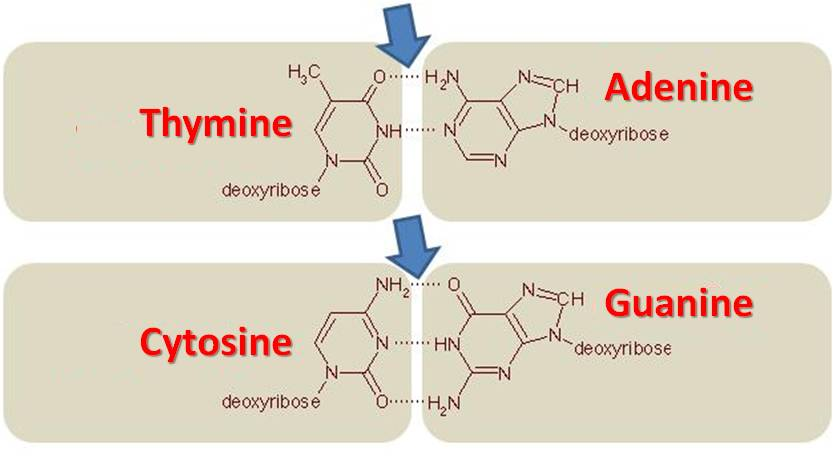
\includegraphics[keepaspectratio=true,scale=0.5]{images/gc_content.jpg}
		\caption{Комлементарные пары: аденин-тимин и гуанин-цитозин}
	\end{figure}
\end{definition}

В случае RNA-seq простой модели, к сожалению, быть не может. Дело в том, что геном статичен. Факторов, которые могут повлиять на распределение ридов в DNA-seq, не так много: это либо структурные вариации, либо особенности нуклеотидной последовательности как строки, без привязки к её биологическому смыслу. Картина экспрессии же постоянно меняется. На неё влияет и клеточный цикл, и окружающая среда, и патологии отдельных компонент клетки. Многочисленные регуляторные механизмы не позволяют моделировать экспрессию генов по отдельности: уровни экспрессии часто коррелируют, а иногда и зависят друг от друга нелинейно (т.н. \textbf{синергия генов}). Хуже того, в науке хорошо изучено такое явление как \textbf{эпистаз} — мутации в одном гене могут приводить к качественным изменениям фенотипа, выходящим далеко за пределы непосредственных функций этого гена. В современной науке существует множество моделей транскрипции, принимающих во внимание многие из этих факторов, но их содержательный обзор выходит далеко за рамки данной работы. 

\subsection{Алгоритмы предобработки данных}
Профессия вычислительного биолога подразумевает рутинную обработку больших гетерогенных данных, особенно что касается single-cell технологий. В связи с этим был реализован протокол предобработки данных секвенирования, основные шаги которого разобраны в данном разделе.
\begin{figure}[H]
	\centering
	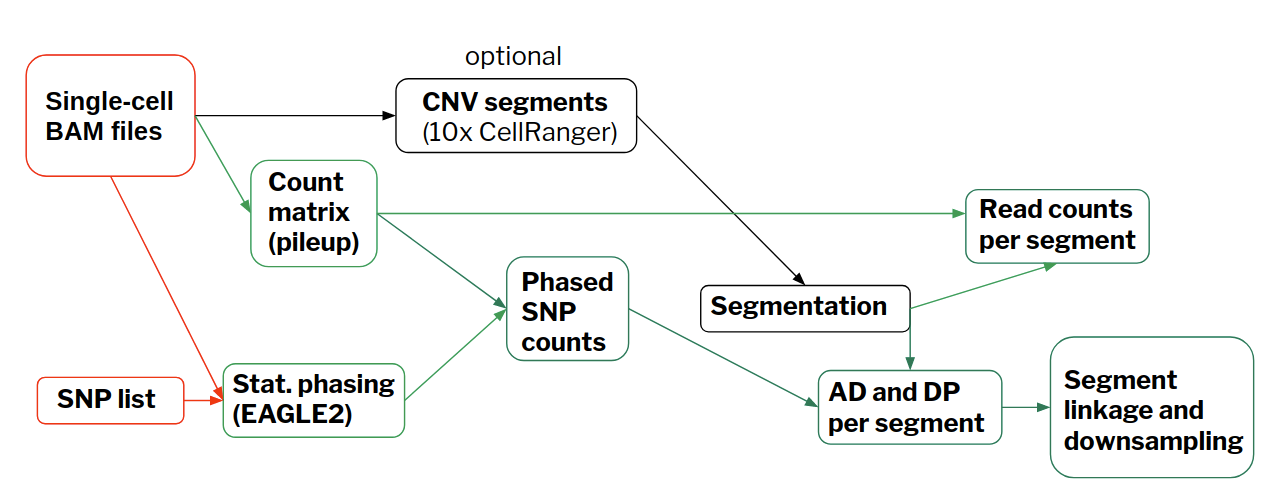
\includegraphics[keepaspectratio=true,scale=0.4]{images/preprocessing_pipeline.png}
	\caption{Граф протокола предобработки данных для алгоритма XClone. Красным обозначены входные данные, чёрным — опциональные шаги, зелёным — реализованные стадии.}
\end{figure}
\subsubsection{Извлечение данных из BAM-файлов}
\textbf{BAM} — \textit{binary SAM — binary sequence alignment/map format} — общепринятый формат сжатого хранения данных секвенирования, c подробностями которого можно ознакомиться в оригинальной публикации \cite{Samtools}. BAM-файл, полученный по протоколам 10x Genomics, занимает до нескольких терабайтов дискового пространства, потому эффективное извлечение информации из BAM-файлов это нетривиальная инженерная задача. Главные входные файлы XClone — матрицы прочтений. Таких матриц требуется три:
\begin{itemize}
	\item матрица $\mathrm{RD}$ всех прочтений достаточного качества;
	\item матрица $\mathrm{DP}$ всех прочтений, накрывающих хоть один ОНП в пределах сегментов; 
	\item матрица $\mathrm{AD}$ всех прочтений, накрывающих хоть альтернативный аллель ОНП в пределах сегментов.
\end{itemize}
Для получения матрицы $\mathrm{RD}$ из данных scRNA-seq был использован протокол \textbf{count} из \textbf{CellRanger}. Для всех остальных матриц во всех остальных случаях был использован \textbf{CellSNP}\footnote{https://github.com/single-cell-genetics/cellSNP}. 
\subsubsection{Статистическое фазирование гаплотипов} 
Гаплотипирование — определение того, от какого родителя унаследован каждый алллель в геноме — одна из ключевых задач генетики человека. Сложность её решения обусловлена контекстом, в котором она возникает в современных исследованиях, когда секвенируются порядка $2\cdot 10^{4}$ — $10^{6}$ позиций в геномах тысяч человек. Если прочтения короткие и не накрывают много позиций одновременно, то нужно секвенировать обоих родителей каждого участника эксперимента, что непрактично и не всегда возможно. Следовательно, нужно разрабатывать статистические методы гаплотипирования. Они основаны на наблюдении, что некоторые группы аллелей часто наследуются совместно. Это явление называется \textbf{неравновесной сцепленностью}. Если прогаплотипировано достаточное количество представителей популяции, то можно построить приближённые таблицы сцепленности и гаплотипировать новые образцы методом максимизации правдоподобия. 

На момент написания этого текста, стандартом статистического гаплотипирования считается алгоритм \textbf{EAGLE2}\cite{Eagle2}\footnote{https://data.broadinstitute.org/alkesgroup/Eagle/}. Этот алгоритм основан на скрытых марковских моделях и использует 32,470 образца из базы данных \textbf{Haplotype Reference Consortium}\cite{HaplotypeReferenceConsortium}.

Алгоритм EAGLE2 обладает существенным недостатком: его метки имеют только локальный смысл. В пределах окна в 20-50 килобаз любые два ОНП с одинаковой наследуются совместно, но при сдвиге окна смысл меток может спонтанно поменяться на противоположный, это так называемая \textbf{ошибка смены цепи}. Т.е. два ОНП с разных концов хромосомы, помеченые одной меткой, могут быть унаследованы от разных родителей. Из-за этого в матрицах прочтений размывается сигнал аллельного дисбаланса: чтобы сделать данные менее разреженными, прочтения соседних небольших сегментов суммируются, в том числе и аллель-специфичные. Ясно, что если среди двух соседних сегментов с одинаковой меткой один полностью унаследован от отца, а второй — от матери, то при сложении их аллель-специфичные сигналы скомпенсируют друг друга. Это, в свою очередь, приводит к неправильному предсказанию аллель-специфичных структурных вариаций и неправильной кластеризации клеток. Авторы EAGLE2 в переписке явно дали понять, что в общем случае  детектировать и исправлять такого рода ошибки их подход не позволяет. Но в контексте модели XClone удалось разработать статистический метод, показавший хорошие результаты при устранении ошибок смены цепи. Его подробное описание можно найти в одноимённом разделе.

\subsubsection{Подходы к сегментации генома}
Одной из основных задач XClone является предсказание \textbf{ASCNV} — аллель-специфических структурных вариаций генома. Это происходит в несколько этапов: (1) вначале производится сегментация генома с одновременным подсчётом матриц прочтений, (2) затем глубина покрытия сегментов сравнивается с эталонной для подсчёта RDR, (3) откуда получается оценка общего числа копий, (4) которая затем уточняется при помощи сигналов аллельного дисбаланса. Тем не менее, на точность предсказания влияют ещё и технические факторы, фигурирующие в вероятностной модели числа прочтений. Наиболее существенным фактором является bin mappability.

Подсчёт bin mappability — задача чисто техническая и довольно утомительная, т.к. она подразумевает проведение симуляций процесса секвенирования по какому-то конкретному протоколу. Кроме того, она давно считается решённой, а потому не представляет особого научного интереса. В связи с этим, для отфильтровывания участков низкого качества используется готовое решение — \textbf{CellRanger DNA}, алгоритм\footnote{https://support.10xgenomics.com/single-cell-dna/software/pipelines/\\latest/algorithms/cnv\_calling} от 10X Genomics, поставщика оборудования для single-cell севенирования в научной группе автора. Этот алгоритм разбивает геном на сегменты длиной в 20кб, после чего отфильтровывает те, для которых bin mappability меньше, чем 70\% (не более 10-15\% при использовании референсного генома GRCh37). CellRanger DNA сам по себе является алгоритмом поиска CNV. Тем не менее, он размечает максимально возможную часть генома каждой из клеток, в том числе участки без структурных вариантов. Благодаря этому можно гарантировать, что все участки генома, пригодные для надёжного определения ASCNV, войдут в итоговую сегментацию. 

Найденные участки накрывают некоторое подмножество референсного генома, которое затем подразделяется на сегменты размера 20-50 килобаз, в пределах которых вероятность ошибки смены цепи невелика, а потому сигнал аллельного дисбаланса статистически достоверный.

\begin{figure}[H]
	\centering
	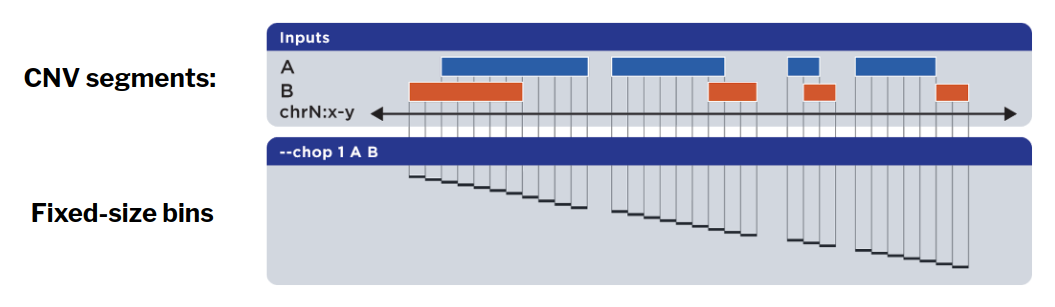
\includegraphics[keepaspectratio=true,scale=0.4]{images/segmentation.png}
	\caption{Иллюстрация алгоритма сегментирования генома. Длина индивидуальных сегментов задаётся заранее и выбирается из диапазона 20-50кб. Каждые $ k $ подряд идущих фрагментов затем объединяются в блоки. Соответствующие подматрицы прочтений при этом суммируются с одновременной коррекцией ошибок смены цепи.}
\end{figure}

В силу того, что структурные вариации обычно охватывают участки генома размеров хотя бы в несколько мегабаз, перед началом предсказания уместно аггрегировать подряд идущие сегменты в блоки фиксированного размера (обычно 1-5 мегабаз), чтобы получить менее шумные BAF и RDR. Тем не менее, наивно аггрегировать содержимое сегментов внутри блока — просуммировать числа прочтений — не получится, т.к. можно потерять аллель-специфический сигнал из-за ошибок смены цепи. В связи с этим был разработан алгоритм суммирования с коррекцией ошибок, который разобран в следующем разделе.

Такой подход к сегментации генома используется в заключительной версии XClone. Тем не менее, изначально большие надежды возлагались на более продвинутый метод, основанный на данных секвенирования длинными прочтениями по технологии Oxford Nanopore. 

\subsubsection{Исправление ошибок смены цепи}
Поскольку одной из главных задач XClone является предсказание \textit{аллель-специфичных} структурных вариаций в геноме, матрицы $\mathrm{AD}$ и $\mathrm{DP}$ аллель-специфичных прочтений должны отражать биологию аллельного дисбаланса в клетках образца. Для этого нужно понимать, к какому гаплотипу принадлежит каждый ОНП. В разделе про статистическое гаплотипирование ОНП был сделан акцент на том, что существующие алгоритмы гарантируют только локальную корректность: при использовании алгоритма EAGLE2, следует ожидать, что при разбиении хромосомы на непересекающиеся окна длины 20-50 килобаз все гетерозиготные ОНП в пределах одного окна будут иметь одинаковый гаплотип, если это на самом деле так. Тем не менее, гаплотипы соседних сегментов с точки зрения алгоритма могут не совпадать даже тогда, когда на самом деле должны. К этому приводят так называемые \textbf{ошибки смены цепи} (\textit{switching error}) — спонтанная и неявная замена гаплотипических меток на противоположные внутри алгоритма. Классификацию ошибок смены цепи можно найти в статье \cite{Choi2018Plos}, цитата из которой приведена ниже:

\textit{"Phasing accuracy is typically measured by counting the number of \textbf{‘switches’} between known maternal and paternal haplotypes that should not occur if individual maternal and paternal chromosomal nucleotide sequence content has been accurately characterized. If an inconsistency is identified, then it is called a ‘switch error.’ These switch errors manifest themselves as induced and false recombination events in the inferred haplotypes compared with the true haplotypes. To identify \textbf{switch errors}, the phase of each site is compared with upstream neighboring phased sites. The switch error rate (SER) is defined as the number of switch errors divided by the number of opportunities for switch errors. Switch errors were further classified into three categories: \textbf{long}, \textbf{point}, and \textbf{undetermined}. A long switch appears as a large-scale pseudo recombination event; that is, there are no other switches in the local neighborhood around the long switch (e.g., no other switches within three consecutive heterozygous sites). On the contrary, a small-scale switch error appearing as two neighboring switch errors is considered as a point switch (e.g., two switches within three consecutive heterozygous sites, with the pair of switches counted as a point switch). The remaining switches are considered undetermined (e.g., only two sites phased in a small phasing block, so the switch error could not be classified into long or point)."}

Тем не менее, разбиение генома на фрагменты по 20-50 килобаз непрактично: в силу разреженности данных, это даёт  слабый и зашумленный сигнал аллельного дисбаланса. В связи с этим был разработан метод, одновременно решающий обе описанные проблем. На первом шаге алгоритма происходит разбиение генома на непересекающиеся сплошные сегменты длины $L$. Затем каждые $N$ подряд идущих сегментов объединяются в блок длины $NL$. В пределах блока переключения моделируются бернуллиевскими случайными величинами, по одной на каждый сегмент. Параметры этих распределений, в свою очередь, выводятся \textbf{ЕМ-алгоритмом}. После исправления ошибок, прочтения сегментов внутри блока суммируются, что даёт более стабильный сигнал. Эта идея была сформулирована в \cite{ChiselBiorxiv}, но технические детали были осознанно исключены авторами CHISEL из препринта. 

Прежде чем приступать к рассмотрению метода, сформулируем необходимые определения:

\begin{definition}[\textit{ЕМ-алгоритм}]$  $\\
EM-алгоритм (от английского \textit{"EM"} — \textit{"Expectation Maximization"}) — метод поиска оценок максимального правдоподобия (ОМП) или оценок апостериорного максимума (ОАП) параметров статистических моделей, содержащих скрытые переменные. 

\begin{algorithm}[H]
	\SetAlgoLined
	\KwResult{$\bm{\Theta}^{\ast},\ p(\bm{Z}\ |\ \bm{X}, \bm{\Theta}^{\ast})$}
	\text{$t = 0$}\;
	\text{$\bm{\Theta}^{(0)}$ инициализируется случайно}\;
	\While{$Q(\bm{\Theta}^{(t+1)}\ |\ \bm{\Theta}^{(t+1)}) - Q(\bm{\Theta}^{(t)}\ |\ \bm{\Theta}^{(t)}) > \eps$}{
		$\mathcal{L}(\bm{\Theta}^{(t)}; \bm{Z}, \bm{X}) := p(\bm{X}, \bm{Z}\ |\ \bm{\Theta}^{(t)})$\;
		$Q(\bm{\Theta}\ |\ \bm{\Theta}^{(t)}) := \mathbb{E}_{\bm{Z} | \bm{X}, \bm{\Theta}^{(t)}} \log \mathcal{L}(\bm{\Theta}; \bm{Z}, \bm{X})$ \tcp{E-шаг}
		$\bm{\Theta}^{(t+1)} := \arg\max\limits_{\bm{\Theta}} Q(\bm{\Theta}\ |\ \bm{\Theta}^{(t)})$ \tcp{M-шаг}
		$t = t + 1$
	}
	$\bm{\Theta}^{\ast} := \bm{\Theta}^{(t)}$
	\caption{ЕМ-алгоритм в общем виде}
\end{algorithm}

Здесь $\bm{Z}$ — дискретные скрытые переменные, $\bm{\Theta}$ — параметры статистической модели, $\bm{X}$ — выборка, $\eps > 0$, $p$ — функция плотности. Каждая итерация алгоритма состоит из двух основных шагов:
\begin{enumerate}
	\item \textbf{Е-шаг}, на котором устраняется явная зависимость от скрытых переменных посредством взятия матожидания логарифма совместной функции правдоподобия по условному распределению $\bm{Z}\ |\ \bm{X}, \bm{\Theta}^{(t)}$;
	\item \textbf{M-шаг}, на котором параметры нового апостериорного распределения $\bm{\Theta}^{(t+1)}$ выбираются таким образом, чтобы максимизировать $ Q(\bm{\Theta}, \bm{\Theta}^{(t)}) $ — функцию правдоподобия "в среднем". 
\end{enumerate}
\end{definition}

С теоретическим обоснованием и формальным доказательством корректности EM-алгоритма можно ознакомиться в (\cite{MurphyProbabilisticML}, стр. 363-365). В контексте решаемой задачи $\bm{X}, \bm{Z}, \bm{\Theta}$ имеют следующий смысл:
\begin{itemize}
	\item $\bm{Z} = \{z_{1}, \ldots, z_{N}\}$ — независимые в совокупности индикаторы корректности гаплотипов сегментов
	\begin{gather*}
			\forall i: z_i \sim \mathrm{Bern}(p_i)\\
			\forall q \in \{0, 1\}^{N}: p(\bm{Z} = q\ |\ p_1, \ldots, p_n) = \prod_{i=1}^{N} p(z_i = q_i\ |\ p_i) = \prod_{i=1}^{N} p_i^{q_i} ( 1 - p_i)^{1-q_i}
	\end{gather*}
	Если $z_i = 1$, то будем говорить, что сегмент $i$ имеет корректный гаплотип, иначе — инвертированный. Эти обозначения имеют смысл только в пределах одного блока, в соседних блоках метки могут иметь противоположный смысл. Из этого наблюдения становится ясно, что алгоритм не решает проблему переключения полностью, но уменьшает число ошибок за счёт аггрегации сегментов в блоки.
	\item Обозначим через $M$ число клеток образца, тогда $\bm{X} = (\bm{X}_{1}, \ldots, \bm{X}_{M}),\ X_{c} := (\bm{a}_c, \bm{b}_c)$ —  вектора прочтений для каждой из клеток, по компоненте на сегмент.  $\bm{a}_c = (a_{c, 1}, \ldots, a_{c, N})$ — число прочтений аллеля А (альтернативный аллель), $\bm{b}_c =  (b_{c, 1}, \ldots, b_{c, N})$ — аллеля Б (референсный аллель).
	\item $\forall c \in \overline{1, M}: \bm{r}_c := \bm{a}_{c} + \bm{b}_{c}$ — вектора прочтений обоих аллелей вместе.
	\item $\bm{\Theta} = (\theta_1, \ldots, \theta_M; p_1, \ldots, p_N)$, где $\theta_c$ — пропорция ридов гаплотипа 1 в блоке в клетке $c$. Алгоритм предполагает, что пропорция гаплотипа 1 одинакова во всех сегментах внутри блока с точностью до переключения.
\end{itemize}
	
В этих обозначениях можно сформулировать и доказать следующее утверждение:
\begin{claim}
	Правила пересчёта параметров апостериорного распределения на М-шаге ЕМ-алгоритма имеют вид:
	\begin{equation}
		\begin{aligned}
			p_{i}^{(t+1)} &= \dfrac{ p_{i}^{(t)} \prod_{c=1}^{M} (\theta_{c}^{(t)})^{a_{c, i}} (1 - \theta_{c}^{(t)})^{b_{c, i}}}{p_{i}^{(t)} \prod_{c=1}^{M} (\theta_{c}^{(t)})^{a_{c, i}} (1 - \theta_{c}^{(t)})^{b_{c, i}} + (1 - p_{i}^{(t)}) \prod_{c=1}^{M} (\theta_{c}^{(t)})^{b_{c, i}} (1 - \theta_{c}^{(t)})^{a_{c, i}}}\\
			\theta_c^{(t+1)} &= \frac{\sum_{i=1}^{N}a_{i,c} \gamma^{(t)}_{i,1} + b_{i,c} \gamma^{(t)}_{i,0}}{\sum_{i=1}^{N} r_{i,c}}
		\end{aligned}
		\label{em_update_rules}
	\end{equation}
	где $\forall j \in \{0, 1\}: \gamma^{(t)}_{i,j} := P(z_i = j\ |\ \bm{X}, \bm{\Theta}^{(t)})$.
\end{claim}
\begin{proof}
  Вектора прочтений в клетках независимы в совокупности, потому: 
	\begin{gather*}
			P(\bm{X}\ |\ \bm{Z}, \bm{\Theta}) = \prod_{c=1}^{M} p(\bm{X}_c\ |\ \bm{Z}, \bm{\Theta}) = \prod_{c=1}^{N} \theta_{c}^{\widehat{a}_c(\bm{Z})}(1 - \theta_{c})^{\widehat{b}_c(\bm{Z})}
	\end{gather*}
	Где 
	\begin{gather*}
	\begin{cases}
		\widehat{a}_c(\bm{Z}) := \sum_{i=1}^{N} \left[z_i a_{c, i} + (1 - z_i) b_{c, i} \right],\\
		\widehat{b}_c(\bm{Z}) := \sum_{i=1}^{N} \left[(1 - z_i) a_{c, i} + z_i b_{c, i} \right],\\
		c \in \overline{1, M}
	\end{cases}
	\end{gather*}
	Тогда функция правдоподобия и её логарифм принимают вид
	\begin{align*}
			&\mathcal{L}(\bm{\Theta}; \bm{X}, \bm{Z}) = p(\bm{X}, \bm{Z} \ |\ \bm{\Theta}) = p(\bm{X}\ |\ \bm{Z}, \bm{\Theta}) p(\bm{Z}\ |\ \bm{\Theta})\\
			&l(\bm{\Theta}; \bm{X}, \bm{Z}) = \log \mathcal{L}(\bm{\Theta}; \bm{X}, \bm{Z}) =\\
			&= \log \prod_{\bm{q} \in \{0, 1\}^{N}} \left(\prod_{c=1}^{M} \theta_{c}^{\widehat{a}_c(\bm{q})}(1-\theta_{c})^{\widehat{b}_c(\bm{q})} \prod_{i=1}^{N} p_i^{q_i}(1-p_i)^{1-q_i}\right)^{\mathbb{I}\{\bm{Z} = \bm{q}\}} =\\
			&=\sum_{\bm{q} \in \{0, 1\}^{N}} \mathbb{I}\{\bm{Z} = \bm{q}\} \left( \sum_{c=1}^{M}\sum_{i=1}^{N} \widehat{a}_{c,i}(\bm{q}) \log \theta_{c} + \widehat{b}_{c,i}(\bm{q}) \log (1-\theta_{c})\right) +\\
			&+ \sum_{\bm{q} \in \{0, 1\}^{N}} \mathbb{I}\{\bm{Z} = \bm{q}\} \left(\sum_{i=1}^{N} q_{i} \log p_{i} + (1 - q_{i}) \log (1 - p_{i}) \right)
	\end{align*}
	Изменением порядка суммирования можно показать, что каждая из этих двух сумм распадается на $N$ сумм поменьше, по одной на каждую из скрытых переменных. В следствие этого и того, что компоненты случайного вектора $ \bm{Z} $ независимы в совокупности, шаги EM-алгоритма имеют вид:\\
	\noindent \textbf{E-шаг:}
	\begin{align*}
		&p(\bm{Z}\ |\ \bm{X}, \bm{\Theta}^{(t)})\ \propto\ p(\bm{X}\ |\ \bm{Z}, \bm{\Theta}^{(t)}) p(\bm{Z}\ |\ \bm{\Theta}^{(t)}) \implies\\
		&\implies \E_{\bm{Z}|\bm{X}, \bm{\Theta}^{(t)}} l(\bm{\Theta}; \bm{Z}, \bm{X}) = \sum_{i=1}^{N} \E_{\bm{z}_i|\bm{X}_i, \bm{\Theta}^{(t)}} \log \mathcal{L}(\bm{\Theta}; \bm{z}_i, \bm{X}_i) =\\
		&= \sum_{i=1}^{N} \sum_{q_i = 0}^{1} p(\bm{z}_i = q_i\ |\ \bm{X}_i, \bm{\Theta}^{(t)}) \left(
		\begin{aligned}
			&\sum_{c=1}^{M} \left[ \widehat{a}_{c,i}(q_i) \log \theta_{c} + \widehat{b}_{c,i}(q_i) \log (1 - \theta_{c}) \right] +\\
			&+ \log p(\bm{z}_i = q_i\ |\ \bm{\Theta})
		\end{aligned} \right) =\\
		&= \sum_{i=1}^{N} \left[ 
		\begin{aligned}
			&\gamma_{i,1}^{(t)} \left( \sum_{c=1}^{M} \left[a_{c,i} \log \theta_c + b_{c,i} \log(1-\theta_c) \right] + \log p_i \right) +\\ 
			&+ \gamma_{i,0}^{(t)} \left( \sum_{c=1}^{M} \left[b_{c,i} \log \theta_c + a_{c,i} \log(1-\theta_c) \right] + \log (1 - p_i) \right) 
		\end{aligned}
		\right] = Q(\bm{\Theta}\ |\ \bm{\Theta}^{(t)})
	\end{align*}
	
	\noindent \textbf{M-шаг:}
	\begin{gather*}
		p_{i}^{(t+1)} = \arg\max_{p_{i}} Q(\bm{\Theta}\ |\ \bm{\Theta}^{(t)}) \iff \frac{\gamma_{i, 1}^{(t)}}{p_{i}^{(t+1)}} - \frac{\gamma_{i, 0}^{(t)}}{1 - p_{i}^{(t+1)}} = 0 \iff p_{i}^{(t+1)} = \gamma_{i, 1}^{(t)}\\
		\begin{aligned}
			\theta_{c}^{(t+1)} = \arg\max_{\theta_c} Q(\bm{\Theta}\ |\ \bm{\Theta}^{(t)}) &\iff \frac{\sum_{i=1}^{N} \gamma_{i,1}^{(t)} a_{c, i} + \gamma_{i,0}^{(t)} b_{c, i}}{\theta_{c}^{(t+1)}} - \frac{\sum_{i=1}^{N} \gamma_{i,1}^{(t)} b_{c, i} + \gamma_{i,0}^{(t)} a_{c, i}}{1 - \theta_{c}^{(t+1)}} = 0\\
			&\iff \theta_c^{(t+1)} = \frac{\sum_{i=1}^{N} \gamma_{i,1}^{(t)} a_{c, i} + \gamma_{i,0}^{(t)} b_{c, i}}{\sum_{i=1}^{N} a_{c, i} +  b_{c, i}}
		\end{aligned}
	\end{gather*}
	Где необходимое условие локального экстремума является также достаточным в силу выпуклости функции $Q(\bm{\Theta}\ |\ \bm{\Theta}^{(t)})$ (\cite{MurphyProbabilisticML}, стр. 363-364).
\end{proof}

\begin{figure}[H]
	\centering
	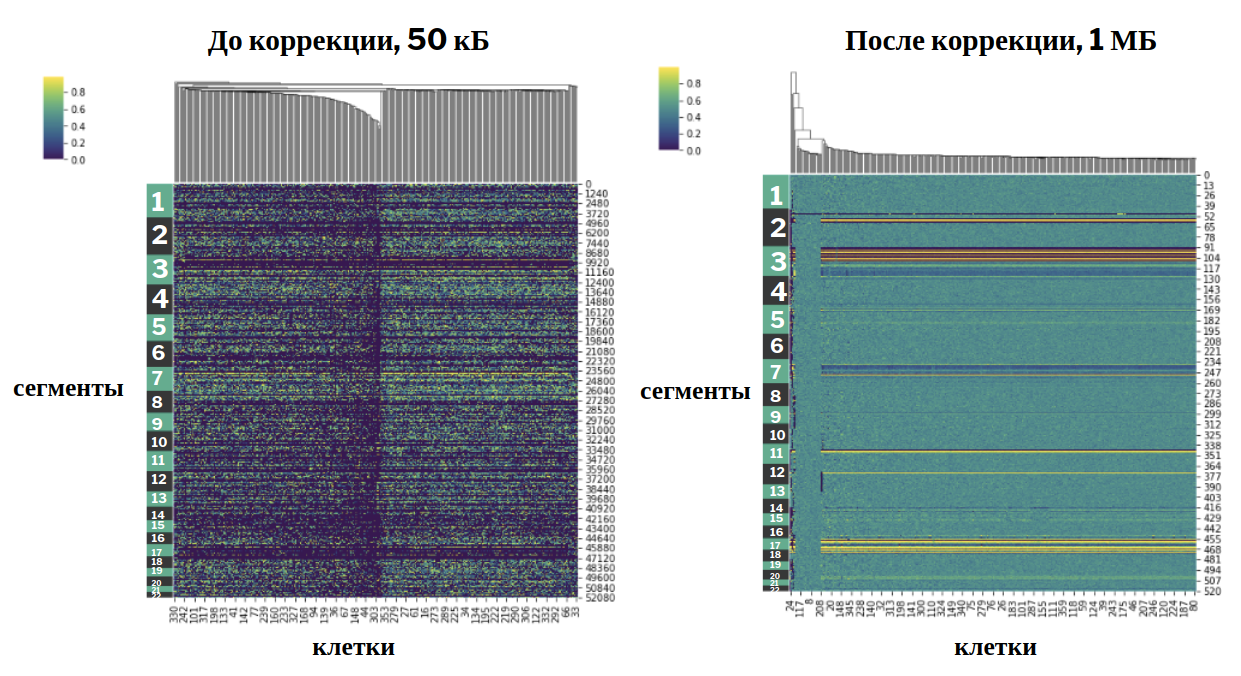
\includegraphics[keepaspectratio=true,scale=0.4]{images/bin_linkage.png}
	\caption{Коррекция ошибок смены цепи на примере ДНК-образца STP-Nuclei. На рисунке изображены тепловые карты долей аллеля из <<материнского>> гаплотипа, числа слева обозначают номер хромосомы. Картина аллельного дисбаланса до коррекции практически не прослеживается, после — становится очевидна.}
\end{figure}

После того, как значения $z_1, \ldots, z_N$ были определены по данным DNA-seq, их же можно использовать для предобработки данных RNA-seq, полученных из образцов тканей того же пациента. Это даёт возможность интеграции двух модальностей в единую статистическую модель.

Стоит отметить, что на практике $p_{i}^{(t+1)}$ следует считать по эквивалетной, но уже численно устойчивой формуле:
\begin{gather*}
	p_{i}^{(t+1)} = \left(1 + \exp\left[\log(1 - p_{i}^{(t)}) - \log(p_{i}^{(t)}) + \sum_{c=1}^{M} \Delta_{c, i} (\log(\theta_{c}^{(t)}) - \log(1 - \theta_{c}^{(t)}))\right]\right)^{-1}
\end{gather*}
Где $\Delta_{c, i} := b_{c, i} - a_{c, i}$, а показатель экспоненты стоит искусственно приводить к диапазону $[-C; C]$ для некоторого $C > 0$ (авторами было выбрано $C = 100$). В противном случае $\prod_{c=1}^{M} (\theta_{c}^{(t)})^{a_{c, i}} (1 - \theta_{c}^{(t)})^{b_{c, i}}$ может представлять собой произведение тысяч или даже миллионов очень маленьких величин в больших степенях. Стандартной реализации чисел с плавающей запятой двойной точности недостаточно для хранения результатов промежуточных вычислений при использовании наивной формулы. 
\subsection{Использованные данные}
\subsection{Первоначальная версия XClone: только ASE-модуль}

\subsubsection{Plate notation}
\subsubsection{Семплирование по Гиббсу}
\subsubsection{Предложенная модель, её недостатки}
\textbf{scDNA + CNV and scRNA, different samples}

\begin{figure}[h!]
	\centering
	\tikz{ %
		\node[obs] (nu) {${\nu_{l}}$}; %
		\node[latent, below=of nu] (Theta) {${\theta_{il}}$}; %
		\node[latent, fill=blue!20, left =of nu, xshift=-0.5cm] (I_G) {${I_{j}^G}$}; %
		\node[latent, right=of nu, xshift=0.5cm] (I_E) {${I_{h}^E}$}; %
		
		\node[latent, rectangle, below=of I_G] (P_G) {${p_{ij}^G}$} ; %
		\node[latent, rectangle, below=of I_E] (P_E) {${p_{ih}^E}$} ; %
		
		\node[latent, fill=blue!20, below=of Theta] (T) {${t_{ik}}$} ; %
		\node[obs, below=of P_G] (A_G) {${a_{ij}^G}$} ; %
		\node[obs, below=of P_E] (A_E) {${a_{ih}^E}$} ; %
		\node[obs, left=of A_G] (D_G) {${d_{ij}^G}$} ; %
		\node[obs, right=of A_E] (D_E) {${d_{ih}^E}$} ; %
		
		\edge {nu} {Theta} ; %
		\edge {I_G} {P_G} ; %
		\edge {I_E} {P_E} ; %
		\edge {Theta} {P_G} ; %
		\edge {T} {P_G} ; %
		\edge {Theta} {P_E} ; %
		\edge {T} {P_E} ; %
		\edge {P_G} {A_G} ; %
		\edge {D_G} {A_G} ; %
		\edge {P_E} {A_E} ; %
		\edge {D_E} {A_E} ; %
		
		
		{\tikzset{plate caption/.append style={below=5pt of #1.south east}};
			\plate[inner xsep=0.8cm, inner ysep=0.4cm, xshift=-0.6cm, yshift=0cm] {plate1} {(D_G) (A_G)(P_G)(D_E) (A_E)(P_E)} {CNV-haplo block $i$} };
		
		{\tikzset{plate caption/.append style={below=30pt of #1.south}};
			\plate[inner xsep=0.4cm, inner ysep=0.4cm, xshift=0.1cm, yshift=0.28cm, color=black] {plate1} {(D_G) (A_G)(P_G)(I_G)} {cell $j$ in scDNA} };
		{\tikzset{plate caption/.append style={below=30pt of #1.south}};
			\plate[inner xsep=0.4cm, inner ysep=0.4cm,  xshift=-0.1cm, yshift=0.28cm, color=black] {plate2} {(D_E) (A_E)(P_E)(I_E)} {cell $h$  in scRNA} };
		
		{\tikzset{plate caption/.append style={above=2pt of #1.north}};
			\plate[inner sep=0.25cm, xshift=0cm, yshift=0.12cm] {plate3} {(nu) (Theta)} {CNV $l$} };
		
		{\tikzset{plate caption/.append style={below=30pt of #1.south}};
			\plate[inner xsep=0.25cm, inner ysep=0.4cm,  xshift=0cm, yshift=0.2cm] {plate4} {(T)} {clone $k$} };
		%			
	}
\end{figure}

\begin{figure}[h!]
	\centering
	\tikz{ %
		\node[obs] (T) {$\mathbf{T}$}; %
		\node[latent, below=of T] (Theta_g) {$\mathbf{\Theta^{G}}$} ; %
		
		\node[obs, left=of T] (I_g_prime) {$\mathbf{I^{G'}}$}; %
		\node[latent, right=of T] (I_g) {$\mathbf{I^{G}}$}; %
		\node[latent, left=of Theta_g] (X_g_prime) {$\mathbf{X^{G'}}$}; %
		\node[latent, right=of Theta_g] (X_g) {$\mathbf{X^{G}}$}; %
		
		\node[obs, below=of X_g_prime] (A_g_prime) {$\mathbf{A^{G'}}$}; %
		\node[obs, left=of A_g_prime] (D_g_prime) {$\mathbf{D^{G'}}$}; %
		\node[obs, below=of X_g] (A_g) {$\mathbf{A^{G}}$}; %
		\node[obs, right=of A_g] (D_g) {$\mathbf{D^{G}}$}; %
		
		\edge {Theta_g} {X_g}; %
		\edge {Theta_g} {X_g_prime}; %
		
		% \edge {T} {Theta_g};  % turned off by YH
		\edge {T} {X_g_prime};
		\edge {T} {X_g};
		
		\edge {I_g_prime} {X_g_prime}; %
		\edge {I_g} {X_g}; %
		
		\edge {X_g_prime} {A_g_prime} ; %
		\edge {D_g_prime} {A_g_prime} ; %
		
		\edge {X_g} {A_g} ; %
		\edge {D_g} {A_g} ; %
	}
\end{figure}

\noindent In this model, clonal assignment $ \mathbf{I^{G'}} $ of cells in scDNA sample is assumed fixed. For each clone $ k $, for each same-CNV block $ i $ the clonal CNV state $ \mathbf{T}_{i,k} $ is defined to be the most frequent CNV state in that position across all cells assigned to clone $ k $. Clonal assignment $ \mathbf{I^{G}} $ in scRNA sample is learned.\\

\noindent This model learns the clonal structure in scRNA sample using ASE profiles from scDNA.

\textbf{Basic definitions}
\begin{enumerate}
	\item \textbf{Constants:}
	\begin{itemize}
		\item $ M', M $ — number of cells in scDNA and scRNA samples respectively.
		\item $ K $  — estimated number of clones in the sample.
		\item $ N_{G} $ — number of same-CNV blocks in scDNA sample (also used in scRNA sample).
		\item $ T_{\max} $ — maximal possible CNV number. User-defined with the default of 5.
		\item $ \tau $ — set of possible CNV configurations: 
		$$\{\{ (1, 0), (0, 1) \}, \{ (2, 0), (1, 1), (1, 2) \}, \ldots, \{(T_{\max}, 0), \ldots, (0, T_{\max})  \} \}$$ The case of zero CNV number should be treated with care if we can't say for sure whether the part of the chromosome (both arms) is deleted).
	\end{itemize}
	\item \textbf{Other known quantities:}
	\begin{itemize}
		\item $ \mathbf{D^{G'}}, \mathbf{D^{G}} $ — total read counts. To get a count of the block, one simply adds up the counts of the variants within the block. Here we assume that variants are far enough from each other, so that almost no reads overlap two variants at the same time. Otherwise, adding things up wouldn't make sense.
		\item $ \mathbf{A^{G'}},\ \mathbf{A^{G}} $ — same for allele-specific counts.
		\item $ \textbf{f} = (f_1, \ldots, f_K)$ — $K$-dimensional vector of estimated clonal fractions ($ \sum_{i=1}^{K} f_i = 1 $) 
		\item $ \mathbf{T} $ — CNV states of blocks ($\mathbf{T_{i,k}}$ is a CNV state of a block $ i $ in clone $ k $).
	\end{itemize}
	\item \textbf{Inferred quantities:}
	\begin{itemize}
		\item $ \mathbf{\Theta^{G}} $ — allelic rates of variants located within blocks of fixed CNV status. $ \mathbf{\Theta^{G}_{i,t}} $ is an allelic rate of a block $i$ with a CNV status $t$. Set of blocks for each clone is unique. Blocks are ordered as tuples of the form (\textit{block start, block length}).
		\item $ \mathbf{I^{G}} \in [K]^{M} $ — cell-to-clone assignment in scRNA sample.
	\end{itemize}
	\item \textbf{Some notational conventions:}
	\begin{itemize}
		\item Capitalized letter without superscript (like $ \mathbf{\Theta} $) denotes the information for both samples.
		\item $ \mathbf{H^{G'}}, \mathbf{H^{G}} $ — CNV status of the blocks in accordance with the current label assignment: 
		$$ 
			\mathbf{H^{G'}_{i,j}} := \mathbf{T_{i, I^{G'}_{j}}},\quad \mathbf{H^{G}_{i,j}} := \mathbf{T_{i, I^{G}_{j}}}
		$$
		\item  $ \mathbf{X^{G'}},\ \mathbf{X^{G}} $ — a shortcut to simplify the notation: $\mathbf{X^{G'|G}_{i,j}}$ is an allelic rate of a block $ i $ in cell $ j $ based of the current cell-to-clone label assignment.
		$$ 
			\mathbf{X^{G'}_{i,j}} := \mathbf{\Theta^{G}_{i, H^{G'}_{i,j}}},\quad \mathbf{X^{G}_{i,j}} := \mathbf{\Theta^{G}_{i, H^{G}_{i,j}}} 
		$$
	\end{itemize}
\end{enumerate}
\textbf{Generative model formulation}
\begin{itemize}
	\item \textbf{Cell-to-clone assignment posterior:}
	\begin{equation}
		\P(\mathbf{I^{G}_{j}} = k_{0} \ |\  \mathbf{A_{j}}, \mathbf{D_{j}}, \mathbf{f}, \mathbf{\Theta}) =  
		\dfrac{\P(\mathbf{A_j} \ |\  \mathbf{D_j}, \mathbf{I^{G}_{j}} = k_{0}, \mathbf{\Theta}) \P(\mathbf{I^{G}_{j}} = k_{0} \ |\  \textbf{f}) }{\sum\limits_{k=1}^{K}\P(\mathbf{A_j} \ |\  \mathbf{D_j}, \mathbf{I^{G}_{j}} = k, \mathbf{\Theta}) \P(\mathbf{I^{G}_{j}} = k\ |\  \textbf{f}) }
	\end{equation}
	
	\item \textbf{ASE model:}
	\begin{equation}
		\begin{aligned}
			\P(\mathbf{A^{G'}_{i,j}}\ |\ \mathbf{D^{G'}_{i,j}}, \mathbf{\Theta^{G}}) &= \mathrm{Binom}(\mathbf{A^{G'}_{i,j}}\ |\ \mathbf{D^{G'}_{i,j}}, \mathbf{X^{G'}_{i,j}})\\
			\P(\mathbf{A^{G}_{i,j}}\ |\ \mathbf{D^{G}_{i,j}}, \mathbf{\Theta^{G}}) &= \mathrm{Binom}(\mathbf{A^{G}_{i,j}}\ |\ \mathbf{D^{G}_{i,j}}, \mathbf{X^{G}_{i,j}}) 
		\end{aligned}
	\end{equation}
	
	\item \textbf{ASE likelihood (both terms factorize over variants):}
	\begin{equation}
		\begin{aligned}
			\P(\mathbf{A^{G'}_{j}}\ |\ \mathbf{D^{G'}_{j}}, \mathbf{I^{G'}_{j}} = k', \mathbf{\Theta^{G}}) &= \prod_{i=1}^{N_{G}} \mathrm{Binom}(\mathbf{A^{G'}_{j}}\ |\ \mathbf{D^{G'}_{j}}, \mathbf{\Theta^{G}_{i, k}})\\
			\P(\mathbf{A^{G}_{j}}\ |\ \mathbf{D^{G}_{j}}, \mathbf{I^{G}_{j}} = k, \mathbf{\Theta^{G}}) &= \prod_{i=1}^{N_{G}} \mathrm{Binom}(\mathbf{A^{G}_{j}}\ |\ \mathbf{D^{G}_{j}}, \mathbf{\Theta^{G}_{i, k}})
		\end{aligned}
	\end{equation}
	
	\item \textbf{Allelic rate likelihood:} 
	\begin{equation}
		\begin{aligned}
			\mathcal{L}(\mathbf{\Theta}) &= \left (\prod_{j=1}^{M'} \sum_{k'=1}^{K}  \P(\mathbf{A^{G'}_{j}}\ |\ \mathbf{D^{G'}_{j}}, \mathbf{I^{G'}_{j}} = k', \mathbf{\Theta^{G}}) \right ) \times\\
			&\times \left (\prod_{j=1}^{M} \sum_{k=1}^{K}  \P(\mathbf{A_{j}}\ |\ \mathbf{D_{j}}, \mathbf{I^{G}_{j}} = k, \mathbf{\Theta^{G}}) \cdot \P(\mathbf{I^{G}_{j}} = k\ |\ \mathbf{f}) \right ) 
		\end{aligned}
	\end{equation}
	To view the clonal assignment in a Bayesian way, we introduce informative prior $ \mathbf{\nu} $ for $\mathbf{\Theta}$.\\ 
	Using that <<posterior $ \propto $ prior $\times$ likelihood>>, we obtain:
	\begin{equation}
		\begin{aligned}
			&\P(\mathbf{\Theta^{G}}\ |\ \mathbf{A}, \mathbf{D}, \mathbf{f}, \mathbf{\nu}) \propto \P(\mathbf{\Theta}\ |\ \mathbf{\nu}) \times \mathcal{L}(\mathbf{\Theta}) =\\
			&= \prod_{l=1}^{N_{G}} \prod_{t\in\tau} \mathrm{Beta}(\alpha_{l,\tau}^{G}, \beta_{l,\tau}^{G}) \times \mathcal{L}(\mathbf{\Theta})
		\end{aligned}
	\end{equation}
	Parameters $\alpha^{G}_{t}, \beta^{G}_{t}$ are selected in such a way that the mode of $\mathrm{Beta}(\alpha^{G}_{t}, \beta^{G}_{t})$ equals to $ 1 / t $ \footnote{because if we assume that allelic rates only depend on the CNV status $ t $ then those rates could be computed as $ 1 / t $}.
\end{itemize}
\textbf{Selecting a prior for $\mathbf{\Theta^G}$}
CNV state of $t$ hides a plethora of possible configurations: it can mean "$ k $ copies of maternal chromosome and $ t - k $ copies of paternal" for any $ k \in \{0, \ldots, t\} $, all the variants are possible. But they are not equally possible: some are more supported by evidence than the rest. During initialization, for each block in each clone we should find the $ (k, t) $-configuration $ (k_0, t) $, such that $ k_0 / t $ is as close to the observed ASE ratio as possible. Then we choose values $ (\alpha, \beta) $ such that the mode of $ \mathrm{Beta}(\alpha, \beta) $, given by $ (\alpha - 1) / (\alpha + \beta - 2) $, equals to $ k_0 / t $. That means, we must solve the following problem:
$$
\dfrac{\alpha - 1}{\alpha + \beta - 2} = \frac{k_0}{t},\ \alpha \ge 1,\ \beta \ge 1
$$
Let's derive the solution. If $ k_0 = 0 $, it is clear that $ \alpha = 1 $, while any $ \beta > 1 $ works\footnote{Nevertheless, it is not clear which one to choose. As we try to reduce prior bias, let's set it to be equal $ 1 + \eps $  for some reasonable $ \eps > 0 $}. Otherwise:
\begin{equation}
\begin{aligned}
(\alpha - 1) t &= (\alpha + \beta - 2) k_0\\
k_0 \beta &= (t - k_0) \alpha -t + 2 k_0\\
\beta &= \left (\frac{t}{k_0} - 1\right ) \alpha - \left (\frac{t}{k_0} - 2 \right )\\
&\implies \alpha = 1 + \frac{t - 2k_0}{t - k_0},\ \beta = 1
\end{aligned}
\end{equation}
As $ \beta $ is linearly dependent from $ \alpha $, any increase in $ \alpha $ will pull $ \beta $ up, "sharpening" the shape of the distribution and making it more biased, thereby we decided to choose the minimal feasible $ \alpha $.
\textbf{Inference (Gibbs sampler)}
To use a Gibbs sampler, we define conditional probability distribution for each scalar random variable:
\begin{enumerate}
	\item \textbf{Cell-to-clone label assignment:} 
	\begin{equation}
		\begin{aligned}
			\P(\mathbf{I^{G}_j} = k\ |\ \mathbf{I^{G}_{-j}}, \mathbf{A^{G}}, \mathbf{D^{G}}, \mathbf{f}, \mathbf{\Theta^{G}}) 
			&\propto \P(\mathbf{A^{G}_{j}}\ |\ \mathbf{D^{G}_{j}}, \mathbf{I^{G}_{j}} = k, \mathbf{\Theta}^{G}) \cdot \P(\mathbf{I^{G}_{j}} = k\ |\ \mathbf{f}) 
		\end{aligned}
	\end{equation}
	\item \textbf{Allelic rates:}
	Assuming fixed assignment, let's expand the joint likelihood equation: 
	\begin{equation}
	\begin{aligned}
		&\P(\mathbf{\Theta}\ |\ \mathbf{A}, \mathbf{D}, \mathbf{I^{G'}}, \mathbf{I^{G}}, \mathbf{f}, \mathbf{\nu}) \propto\\
		&\propto \left\{\prod_{l=1}^{N_{G}} \prod_{t\in \tau}\mathrm{Beta}(\alpha_{T_{l,t}}^{G}, \beta_{T_{l,t}}^{G}) \right\} 
		\times \left[ \prod_{j=1}^{M'} \P(\mathbf{A^{G'}_{j}}\ |\ \mathbf{D^{G'}_{j}}, \mathbf{I^{G'}_{j}}, \mathbf{\Theta^{G}}) \right] 
		\times \left[\prod_{j=1}^{M} \P(\mathbf{A^{G}_{j}}\ |\ \mathbf{D^{G}_{j}}, \mathbf{I^{G}_{j}}, \mathbf{\Theta^{G}}) \right]  =\\
		&= \left\{\prod_{l=1}^{N_{G}} \prod_{t\in \tau}\mathrm{Beta}(\alpha_{T_{l,t}}^{G}, \beta_{T_{l,t}}^{G}) \right\} 
		\times \left[ \prod_{j=1}^{M'} \prod_{i=1}^{N_{G}} \mathrm{Binom}(\mathbf{A^{G'}_{j}}\ |\ \mathbf{D^{G'}_{j}}, \mathbf{\Theta^{G}_{i, k}}) \right] 
		\times \left[\prod_{j=1}^{M} \prod_{i=1}^{N_{G}} \mathrm{Binom}(\mathbf{A^{G}_{j}}\ |\ \mathbf{D^{G}_{j}}, \mathbf{\Theta^{G}_{i, k}}) \right]  =\\
		&= \prod_{l=1}^{N_{G}} \prod_{t \in \tau} \left[ \mathrm{Beta}(\alpha^{G}_{l,t}, \beta^{G}_{l,t}) \prod_{j'=1}^{M'}\prod_{j=1}^{M} \mathrm{Binom}(\mathbf{A^{G'}_{l,j'}}\ |\ \mathbf{D^{G'}_{l,j'}}, \mathbf{X^{G'}_{l,j'}})^{\mathbb{I} \left\{ \mathbf{H^{G'}_{l,j'}} = t \right\}} \mathrm{Binom}(\mathbf{A^{G}_{l,j}}\ |\ \mathbf{D^{G}_{l,j}}, \mathbf{X^{G}_{l,j}})^{\mathbb{I} \left\{ \mathbf{H^{G}_{l,j}} = t \right\}} \right]
	\end{aligned}
	\end{equation}
	From here we derive update rules for individual allelic rates:
	\begin{equation}
		\mathbf{\Theta^{G}_{l,t}}\ |\ \mathbf{I^{G'}}, \mathbf{I^{G}} \sim \mathrm{Beta}(\alpha^{G}_{l,t} + u^{G}_{l,t}, \beta^{G}_{l,t} + v^{G}_{l,t})
	\end{equation}
	where
	\begin{equation}
	\begin{aligned}
		&u^{G}_{l,t} = \sum_{j'=1}^{M'} \mathbf{A^{G'}_{l,j'}} \cdot \mathbb{I}\left\{ \mathbf{H^{G'}_{l,j'}} = t \right\} +   \sum_{j=1}^{M} \mathbf{A^{G}_{l,j}} \cdot \mathbb{I}\left\{ \mathbf{H^{G}_{l,j}} = t \right\}\\
		& v^{G}_{l,t} =\sum_{j'=1}^{M'} (\mathbf{D^{G'}_{l,j'}} - \mathbf{A^{G'}_{l,j'}}) \cdot \mathbb{I}\left\{ \mathbf{H^{G'}_{l,j'}} = t \right\} + \sum_{j=1}^{M} (\mathbf{D^{G}_{l,j}} - \mathbf{A^{G}_{l,j}}) \cdot \mathbb{I}\left\{ \mathbf{H^{G}_{l,j}} = t \right\}
	\end{aligned}
	\end{equation}
\end{enumerate}

\textbf{Notes}

\begin{figure}[h!]
	\centering
	\tikz{ %
		\node[obs] (T) {$\mathbf{T}$}; %
		\node[latent, below=of T] (Theta_g) {$\mathbf{\Theta}$} ; %
		\node[obs, left=of T] (I_g_prime) {$\mathbf{I^{G}}$}; %
		\node[latent, right=of T] (I_g) {$\mathbf{I^{E}}$}; %
		\node[latent, left=of Theta_g] (X_g_prime) {$\mathbf{X^{G}}$}; %
		\node[latent, right=of Theta_g] (X_g) {$\mathbf{X^{E}}$}; %
		
		\node[obs, below=of X_g_prime] (A_g_prime) {$\mathbf{A^{G}}$}; %
		\node[obs, left=of A_g_prime] (D_g_prime) {$\mathbf{D^{G}}$}; %
		\node[obs, below=of X_g] (A_g) {$\mathbf{A^{E}}$}; %
		\node[obs, right=of A_g] (D_g) {$\mathbf{D^{E}}$}; %
		
		\edge {Theta_g} {X_g}; %
		\edge {Theta_g} {X_g_prime}; %
		
		% \edge {T} {Theta_g};  % turned off by YH
		\edge {T} {X_g_prime};
		\edge {T} {X_g};
		
		\edge {I_g_prime} {X_g_prime}; %
		\edge {I_g} {X_g}; %
		
		\edge {X_g_prime} {A_g_prime} ; %
		\edge {D_g_prime} {A_g_prime} ; %
		
		\edge {X_g} {A_g} ; %
		\edge {D_g} {A_g} ; %
	}
\end{figure}

\begin{equation*}
	p_{i,j} = \theta_{i,l_j}; l_j=t_{i,{I_j}}
\end{equation*}

\begin{equation*}
	P(a_{i,j}|d_{i,j}, p_{i,j})= \text{Binom}(a_{i,j}; d_{i,j}, p_{i,j})
\end{equation*}
\subsubsection{Восстановление перестановки меток классов при выводе}

\subsection{Заключительная версия XClone: ASE- и RDR-модули}
\subsubsection{Вариационный байесовский вывод}
\subsubsection{Структура ASE-модуля}
In the xclone model, we aim to cluster cells in scRNA-seq data by its copy number variation (CNV) states across many CNV blocks. The similarity between two CNV states are measured at both allelic fraction and expression count levels, which reflects both the maternal and paternal copy numbers $c_t = [c_{t,1}, c_{t,2}]$ for CNV state $t$. The key novelty of xclone is that it allows to integrate additional information on CNV states and the according parameters of allelic fraction and expression count, for example extracting from scDNA-seq data.

Due to different magnitudes of expressions and allelic bias across genes even with the same CNV block,  we define the model at per gene basis. If a CNV block contains multiple genes, we will introduce separate functions to link CNV states for these neighbouring genes.

As most scRNA-seq data has very low coverage, especially for the droplet based protocols, it is hard to accurately estimate the allelic fraction from expression for most individual heterozygous variants. Therefore, we aggregate multiple variants across one gene by using statistical phasing with haplotype reference. This may increase the power of allelic fraction estimation, though we need to avoid multiple counting when one read covering several nearby SNPs. Once again, multiple genes within one CNV block could be further aggregated, through a separate linkage function.


\textbf{Allelic fraction module}
By aggregating multiple SNPs for each gene, we could have observations on $N$ genes across $M$ cells in scRNA-seq data. For gene $i$ in cell $j$, we denote the read (or UMI) count for alternative allele as $a_{i,j}$ and the total depth (i.e., for both alternative and reference alleles) as $d_{i,j}$. Assuming there are $T$ CNV states and for each state $t$ the maternal and paternal copy number vector $c_t=[c_{t,1}, c_{t,2}]$. If gene $i$ in cell $j$ is in CNV state $t$, we assume the allelic expression follows a binomial distribution with CNV state specific parameter $\theta_t$, as follows,
\begin{equation}
	p(a_{i,j}|d_{i,j}, \theta_t) = \mathtt{Binom}(a_{i,j}|d_{i,j}, \theta_{i,t}).
	\label{Eq:ASE-base}
\end{equation}

Let $A$ and $D$ respectively denote the gene-by-cell count matrices for the alternative allele and the total read depths, and each cell comes from one of the $K$ clones. If cell $j$ is from clone $k$, the cell identity variable $z_{j,k}=1$ otherwise 0. Also, if gene $i$ in clone $k$ is in CNV state $t$, the corresponding CNV state variable $y_{i,k,t}=1$ otherwise 0. Their according matrix or tensor $Z$ and $Y$ are unknown variables. Now, we could define the likelihood for allelic fraction as follows, TODO
\begin{equation}
	p(A, D | Z, Y, \bm\theta)  = \prod_{i=1}^{N} \prod_{j=1}^{M} \prod_{k=1}^{K}\prod_{t=1}^{T} p(a_{i,j}|d_{i,j}, \theta_{i,t}) ^{z_{j,k} \times y_{i,k,t}}
	\label{Eq:ASE-lik}
\end{equation}

Here, we introduce uniform $\mathtt{Multinomial}$ distribution for $Z$ and $Y$ and $\mathtt{Beta}$ distribution for $\bm\theta$ with default hyper-parameters $\alpha_t = (c_{t,1} + 0.01)$ and $\beta_t = (c_{t,2} + 0.01)$ as follows,
\begin{equation}
	\begin{split}
		p(z_{j,k} = 1|\bm\pi) & = \mathtt{Multinom}(1; \bm\pi_{j}) = \pi_{j,k} \\
		p(y_{i,k,t} = 1|U) & = \mathtt{Multinom}(1; \bm{u}_{i,k}) = u_{i,k,t} \\
		p(\theta_{i,t} | \alpha_t, \beta_t) & = \mathtt{Beta} (\theta_{i,t}| \alpha_t, \beta_t)
	\end{split}
\label{Eq:prior-ASE}
\end{equation}

For a start point, we only consider $T=16$ CNV states: \\
$\{[0,0], [0,1], [0,2], [0,3], [1,0], [1,1], [1,2], [1,3], [2,0], [2,1], [2,2], [2,3], [3,0], [3,1], [3,2], [3,3]\}$

\textbf{Expression count module}
For a particular cell $j$, we assume that the expression counts for $N$ genes follows a $\mathtt{Multinomial}$ distribution with total counts as $d_j=\sum_{i=1}^N d_{i,j}$ and probability vector as $\bm f_j=\{f_{1,j},...,f_{N,j}\}$, hence $\sum_{i=1}^{N} f_{i,j} = 1$. In the case of diploid genome, $f_{i,j}=m_i$.

When CNVs exist in the consensual genome for clone $k$, the amplification factor $\bm \gamma$ needs to take into account, and the probability to observe the read counts for $N$ genes can be expressed as 
\begin{equation}
	\begin{aligned}
		\bm d_{j} &:= [d_{1, j}, \ldots, d_{N, j}]\\
		p(\bm d_{j} | d_{j}, \bm f_{j}) &:= \mathtt{Multinom}(\bm d_{j} | d_j, \bm f_{k});\\
		f_{i,k} &:= \dfrac{\sum_{t=1}^{T} m_i \exp[\gamma_t] P(y_{i,k,t}=1)}{\sum_{b=1}^{N}\sum_{t=1}^{T} m_b \exp[\gamma_t] P(y_{b,k,t}=1)}
	\end{aligned}
\label{Eq:RDR-base}
\end{equation}

As can be seen that the diploid expression profile $\bm m$ is shared by all cells, the likelihood for $M$ cells jointly can be written as follows,
\begin{equation}
\begin{aligned}
p(D | Z, Y, \bm m, \bm\gamma)  & := \prod_{j=1}^{M} \prod_{k=1}^{K} p(\bm d_{j} | d_{j}, \bm f_{k}) ^{z_{j,k}}
\end{aligned}
\label{Eq:RDR-lik}
\end{equation}
Here, we introduce $\mathtt{Dirichlet}(\bm\omega)$ as the prior distribution for $\bm m$, and Gaussian process $\mathtt{GP}(\bm\mu, \Sigma)$ as the prior distribution for $\bm \gamma$. The GP prior has fixed hyper-parameters $\mu_t = \log((c_{t,1} + c_{t,2}) / 2 + \varepsilon)$ for CNV state $t$, where $\varepsilon$ is some reasonably small offset, and the covariance matrix $\Sigma$ is defined by the radial basis function kernel $K(\bm c_t, \bm c_{t\prime})=l_1 \exp\{-l_2[(c_{t,1}-c_{t\prime,1})^2 + (c_{t,2}-c_{t\prime,2})^2]\}$, as follows,
\begin{equation}
	\begin{split}
		\bm m|\bm \omega &\sim \mathtt{Dirichlet}( \bm\omega)\\
		\bm \gamma | \bm\mu, \Sigma &\sim \mathtt{ \mathcal{N}}(\bm\mu, \Sigma) \\
	\end{split}
\label{Eq:prior-RDR}
\end{equation}

\textbf{Posterior and inference}
Now, by combining the allelic fraction and expression count likelihoods and their specific prior distributions, we could have the posterior distribution as follows,
\begin{equation}
	\begin{split}
		p(Z, Y, \bm\theta, \bm m, \bm\gamma | A, D)  & \propto p(Z, Y, \bm\theta, \bm m, \bm\gamma) p(A, D | Z, Y, \bm\theta, \bm m, \bm\gamma) \\
		& = p(Z, Y, \bm\theta, \bm m, \bm\gamma) p(D | Z, Y, \bm m, \bm\gamma) p(A, D | Z, Y, \bm\theta)
	\end{split}
\label{Eq:posterior}
\end{equation}
where the prior distribution is independent for all five variables $\Omega=\{Z, Y, \bm\theta, \bm m, \bm\gamma\}$, hence can be multiplied from Eq (\ref{Eq:prior-ASE}) and Eq (\ref{Eq:prior-RDR}). Similarly, the likelihood term can be multiplied by the two likelihood terms in Eq(\ref{Eq:ASE-lik}) and Eq(\ref{Eq:RDR-base}).

Here, we introduce a variational Bayes to infer the posterior of the five000 unknown variables $p(\Omega|A,D)$. Then the inference problem becomes an optimisation problem for minimising the evidence lower bounder (ELBO), as follows 
\begin{equation}
\mathtt{L}(q) = - \mathcal{KL}(q(\Omega)||p(\Omega)) + \int{ q(\Omega) \log p(A,D|\Omega)} \text{d} \Omega
\end{equation}
where the variational distribution $q(\Omega)$ is in the same form as its prior distribution Eq (\ref{Eq:prior-ASE}) and Eq (\ref{Eq:prior-RDR}), while we aim to optimize their parameters to achive the highest ELBO. The details of the derivations can be found in page 463 in Bishop, PRML 2006 or Vireo paper (TODO: introduce it here).

For the right part, we can split it into the allelic fraction and expression count modules, namely
\begin{equation}
	\begin{split}
		\int{ q(\Omega) \log p(A,D|\Omega)} \text{d} \Omega =  
		& \int{ q(Z, Y, \bm\theta) \log p(A, D | Z, Y, \bm\theta)} \text{d} Z \text{d} Y \text{d} \bm\theta + \\
		& \int{ q(Z, Y, \bm m, \bm\gamma) \log p(D|Z, Y,\bm m, \bm\gamma)} \text{d} \bm m, \text{d} \bm\gamma
	\end{split}
\end{equation}
The allelic fraction module could further analytically written as follows,
\begin{equation}
	\footnotesize
		\begin{split}
		\mathbb{E}_{Z, Y, \bm\theta}[\log p(A,D|Z, Y,\bm\theta)] 
		& = \int{ q(Z, Y, \bm\theta) \log p(A, D | Z, Y, \bm\theta)} \text{d} Z \text{d} Y \text{d} \bm\theta \\ 
		& = \sum_{i=1}^N \sum_{j=1}^M  \sum_{k=1}^K  \sum_{t=1}^T  \left\{ \tilde \pi_{j,k} \tilde u_{i,k,t}  [w_{i,j} + a_{i,j}\varphi(\tilde\alpha) + b_{i,j}\varphi(\tilde\beta) - d_{i,j}\varphi(\tilde\alpha + \tilde\beta) ]  \right\}
	\end{split}
\end{equation}
where $w_{i,j}=\log \binom{d_{i,j}}{a_{i,j}}$ is the logarithm of binomial coefficient, $\varphi(\cdot)$ is the digamma function, and $\tilde \cdot$ is the parameters for variational posterior distributions. This part is identical to Vireo model.

\textbf{Supplementary Materials}
\textbf{Derivation of likelihood equation (3.9, ASE module)}
The allelic fraction module could be analytically derived as follows,
\begin{equation}
	\footnotesize
	\begin{split}
		& \int{ q(Z, Y, \bm\theta) \log p(A, D | Z, Y, \bm\theta)} \text{d} Z \text{d} Y \text{d} \bm\theta \\ 
		& = \mathbb{E}_{Z, Y, \bm\theta}[\log p(A,D|Z, Y,\bm\theta)] \\
		& = \mathbb{E}_{Z, Y, \bm\theta}[\log \prod_{i=1}^{N} \prod_{j=1}^{M} \prod_{k=1}^{K}\prod_{t=1}^{T} p(a_{i,j}|d_{i,j}, \theta_t) ^{z_{j,k} \times y_{i,k,t}}] \\
		& = \mathbb{E}_{Z, Y, \bm\theta}\sum_{i=1}^{N} \sum_{j=1}^{M} \sum_{k=1}^{K}\sum_{t=1}^{T} [{z_{j,k} y_{i,k,t} \log{\mathtt{binom}(a_{i,j}|d_{i,j}, \theta_t)}}] \\
		& = \sum_{i=1}^{N} \sum_{j=1}^{M} \sum_{k=1}^{K}\sum_{t=1}^{T} \mathbb{E}_{Z, Y, \bm\theta}[z_{j,k} y_{i,k,t} \log{\mathtt{binom}(a_{i,j}|d_{i,j}, \theta_t)}] \\
		& = \sum_{i=1}^{N} \sum_{j=1}^{M} \sum_{k=1}^{K}\sum_{t=1}^{T} \mathbb{E}_{Z}[z_{j,k}] \mathbb{E}_{Y}[y_{i,k,t}] \mathbb{E}_{\bm\theta}[\log{\mathtt{binom}(a_{i,j}|d_{i,j}, \theta_t)}] \\
		& = \sum_{i=1}^{N} \sum_{j=1}^{M} \sum_{k=1}^{K}\sum_{t=1}^{T} \left\{ \tilde \pi_{j,k} \tilde u_{i,k,t} \mathbb{E}_{\bm\theta}[\log{\mathtt{binom}(a_{i,j}|d_{i,j}, \theta_t)}]\right\} \\
		& = \sum_{i=1}^N \sum_{j=1}^M  \sum_{k=1}^K  \sum_{t=1}^T  \left\{ \tilde \pi_{j,k} \tilde u_{i,k,t}  [w_{i,j} + a_{i,j}\varphi(\tilde\alpha_t) + b_{i,j}\varphi(\tilde\beta_t) - d_{i,j}\varphi(\tilde\alpha_t + \tilde\beta_t) ]  \right\}
	\end{split}
\end{equation}

The integral on $\mathtt{binom}$ distribution can be derived by the use of digamma function, as follows.
\begin{equation}
	\begin{split}
		& \mathbb{E}_{\theta}[\log{p(a|d, \theta)}] \\
		& = \mathbb{E}_{\theta}[\log{\mathtt{binom}(a; d, \theta)}]\\
		& = \mathbb{E}_{\theta}[\log{\binom{a}{d}} + a\log{\theta} + (d-a)\log{(1-\theta)}] \\
		& = \log{\binom{a}{d}} + a\mathbb{E}_{\theta}[\log{\theta}] + (d-a)\mathbb{E}_{\theta}[\log{(1-\theta)}] \\
		& = \log{\binom{a}{d}} + a\mathbb{E}_{\theta}[\log{\theta}] + (d-a)\mathbb{E}_{1-\theta}[\log{(1-\theta)}] \\
		& = \log{\binom{a}{d}} + a(\varphi(\alpha) - \varphi(\alpha + \beta)) + (d-a) (\varphi(\beta) - \varphi(\alpha + \beta))\\
		& = \log{\binom{a}{d}} + a\varphi(\alpha) + (d-a)\varphi(\beta) - d \varphi(\alpha + \beta)
	\end{split}
\end{equation}
where $\theta \sim \mathtt{Beta}(\alpha, \beta)$ and $1-\theta \sim \mathtt{Beta}(\beta, \alpha)$. By using digamma function $\varphi(\cdot)$, one could easily calculate the logarithm of the geometric mean $\mathbb{E}[\log{\theta}]=\varphi(\alpha) - \varphi(\alpha + \beta)$ (see derivation on wikipedia for Beta distribution).

\textbf{Derivation of likelihood equation (3.9, RDR module)}
\begin{equation}
	\begin{aligned}
		&\int{ q(Z, Y, \bm m, \bm\gamma) \log p(D|Z, Y,\bm m, \bm\gamma)} \text{d} \bm m, \text{d} \bm\gamma =\\
		&= \mathbb{E}_{Z, Y, \bm m, \bm \gamma} \log p(D|Z, Y,\bm m, \bm\gamma)  =\\
		&= (\text{Using eq. } \ref{Eq:RDR-lik}) =\\
		&= \mathbb{E}_{Z, Y, \bm m, \bm \gamma} \left[ \sum_{j=1}^{M}\sum_{k=1}^{K} \log p(\bm d_{j}| d_j, \bm f_{k})^{z_{j,k}} \right] =\\
		&= \sum_{j=1}^{M}\sum_{k=1}^{K} \mathbb{E}_{Z, Y, \bm m, \bm \gamma} \left[ z_{j,k} \cdot \log \left(d_{j}! \prod_{i=1}^{N}
		\frac{\widetilde{f}_{i,k}^{d_{i,j}}}{d_{i,j}!} \right) \right] \propto\\
		&\propto (\text{Dropping out constant terms}) \propto\\
		&\propto \sum_{i=1}^{N}\sum_{j=1}^{M}\sum_{k=1}^{K} \mathbb{E}_{Z, Y, \bm m, \bm \gamma} \left[ z_{j,k} \cdot d_{ij} \log \widetilde{f}_{i,k}\right] =\\
		&= \sum_{i=1}^{N}\sum_{j=1}^{M}\sum_{k=1}^{K} \widetilde{\pi}_{j,k} \cdot d_{ij} \cdot \mathbb{E}_{\bm m, \bm \gamma} \log \widetilde{f}_{i,k} 
	\end{aligned}
	\label{Eq:loglik-derivation-base}
\end{equation}
\subsubsection{Структура RDR-модуля}
\subsubsection{Известные недостатки и планы по их исправлению}

